\documentclass[letterpaper,10pt]{article}
\usepackage[top=2cm, bottom=1.5cm, left=1cm, right=1cm]{geometry}
\usepackage{amsmath, amssymb, amsthm,graphicx}
\usepackage{fancyhdr}
\pagestyle{fancy}

\lhead{\today}
\chead{Meeting 3}
\rhead{Justin Hood}

\newcommand{\Z}{\mathbb{Z}}
\newcommand{\Q}{\mathbb{Q}}
\newcommand{\R}{\mathbb{R}}
\newcommand{\C}{\mathbb{C}}
\newtheorem{lem}{Lemma}

\begin{document}
\begin{enumerate}
\item Consider the matrix equation $A\vec{x}=\vec{b}$, with $A\in \R^{n\times n}$ and $\vec{x},\ \vec{b}\in \R^n$. Now the equation,
\[x_1\vec{a}_1+x_2\vec{a}_2+\ldots +x_n\vec{a}_n=\vec{b} \]
can be written as,
\[\begin{bmatrix}
a_1 & a_2 & \ldots & a_n\\
a_1 & a_2 & \ldots & a_n\\
\vdots & \ddots & \ddots & \vdots\\
a_1 & a_2 & \ldots & a_n
\end{bmatrix} \begin{bmatrix}
x_1\\x_2\\ \vdots\\ x_n
\end{bmatrix}=\begin{bmatrix}
b_1\\ b_2\\ \vdots \\ b_n
\end{bmatrix} \]
Where $A$ is an $n\times n$ matrix whose columns are the coefficients in the matrix equation above.
\item We consider solving for the coefficients of the matrix eqation that solves, 
\[p(x)=c_0+c_1x+c_2x^2+c_3x^3\]
given the points $(-4,\ -21),\ (-2,\ 5),\ (1,\ -16),\ (2,\ -15)$. Our matrix equation is, $X\vec{c}=\vec{p}$. Here, $\vec{p}$ is the column vector of the $y$ coordinates, and $X$ is constructed as,
\[X=\begin{bmatrix}
x_0^0 & x_0^1 & x_0^2 & x_0^3\\
x_1^0 & x_1^1 & x_1^2 & x_1^3\\
x_2^0 & x_2^1 & x_2^2 & x_2^3\\
x_3^0 & x_3^1 & x_3^2 & x_3^3\\
\end{bmatrix} \]
Using python, we construct the matrices as above, and directly solve for the coefficient matrix,
\[\vec{c}=\begin{bmatrix}
-9\\-9\\1\\1
\end{bmatrix} \]
So, we arrive at the function, $p(x)=-9-9x+x^2+x^3$. As a check, we plot the function $p(x)$ as well as the points themselves,
\begin{center}
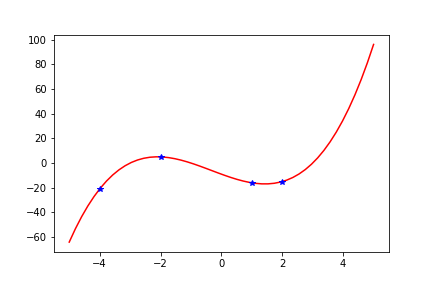
\includegraphics[scale=.7]{2.png}
\end{center}
We see that the function indeed interpolates the data.
\item Considering the points $(-4,\ -21),\ (-2,\ 5),\ (1,\ -16),\ (2,\ -15)$ again, we shall construct the Lagrange interpolating polynomial. First, we construct our $\ell_i$ as,
\begin{align*}
\ell_i &= \prod_{0\leq m \leq k}\frac{x-x_m}{x_j-x_m},\ m\neq j\\
\ell_0 &= \frac{x+2}{-2}\frac{x-1}{-5}\frac{x-2}{-6}\\
\ell_1 &= \frac{x+4}{2}\frac{x-1}{-3}\frac{x-2}{-4}\\
\ell_2 &= \frac{x+4}{5}\frac{x+2}{3}\frac{x-2}{-1}\\
\ell_3 &= \frac{x+4}{6}\frac{x+2}{4}\frac{x-1}{1}
\end{align*}
Our polynomial is then constructed as, $p(x)=\sum_i \ell_iy_i$.
\[p(x)=-21\frac{x+2}{-2}\frac{x-1}{-5}\frac{x-2}{-6}+5\frac{x+4}{2}\frac{x-1}{-3}\frac{x-2}{-4}-16\frac{x+4}{5}\frac{x+2}{3}\frac{x-2}{-1}-15\frac{x+4}{6}\frac{x+2}{4}\frac{x-1}{1}\]
As a check, we again plot the Lagrange polynomial and the points,
\begin{center}
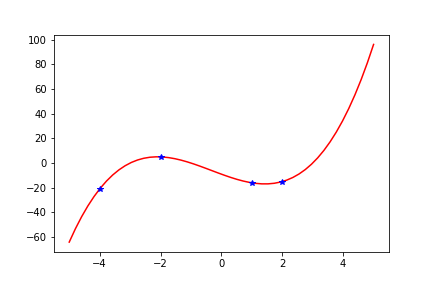
\includegraphics[scale=.7]{3.png}
\end{center}
\item We consider the Lagrange interpolating polynomial between $x_0$ and $x_1$ where $x_1=x_0+h$. Our polynomial construction is,
\begin{align*}
\ell_0 &= \frac{x-x_1}{x_0-x_1}\\
&= \frac{x-(x_0+h)}{x_0-(x_0+h)}\\
&= \frac{x-x_0-h}{-h}\\
\ell_1 &= \frac{x-x_0}{x_1-x_0}\\
&=\frac{x-x_0}{x_0+h-x_0}\\
&=\frac{x-x_0}{h}
\end{align*}
Our function is then,
\[p(x)=f(x_0)\frac{x-x_0-h}{-h}+f(x_1)\frac{x-x_0}{h}\]
Deriving,
\[p'(x)=\frac{f(x_0)}{-h}+\frac{f(x_0+h)}{h}=\frac{f(x_0+h)-f(x_0)}{h}\]
Which is the difference quotient we recall from Calc I.\\
Now, let $x_1=x_0+2h$. Our polynomial construction is,
\begin{align*}
\ell_0 &= \frac{x-x_1}{x_0-x_1}\\
&= \frac{x-(x_0+2h)}{x_0-(x_0+2h)}\\
&= \frac{x-x_0-2h}{-2h}\\
\ell_1 &= \frac{x-x_0}{x_1-x_0}\\
&=\frac{x-x_0}{x_0+2h-x_0}\\
&=\frac{x-x_0}{2h}
\end{align*}
Our function is then,
\[p(x)=f(x_0)\frac{x-x_0-2h}{-2h}+f(x_1)\frac{x-x_0}{2h}\]
Deriving,
\[p'(x)=\frac{f(x_0)}{-2h}+\frac{f(x_0+2h)}{2h}=\frac{f(x_0+2h)-f(x_0)}{2h}\]
Considering that the limit will ignore the coefficient of $2$ in the formula as $h\to 0$, we see that this too will function as a difference quotient as well.
\item Consider the circulant matrix $A$,
\[A=\begin{bmatrix}
2 & -1 & 0 & 0 & 0 & \ldots & -1\\
-1 & 2 & -1 & 0 & 0 & \ldots & 0\\
0 & -1 & 2 & -1 & 0 & \ldots & 0\\
0 & 0 & -1 & 2 & -1 & \ldots & 0\\
0 & 0 & 0 & -1 & 2 & \ldots & 0\\
\vdots & \vdots & \vdots & \vdots & \vdots & \ddots & \vdots\\
-1 & 0 & 0 & \ldots & 0 & -1 & 2
\end{bmatrix} \]
We consider the nullspace of the matrix. To find a vector in the nullspace, we consider the rows of the circulant matrix. Note, that the sum of each row is zero. So, we see that if we consider a vector of constants, i.e., $\lambda \textbf{1}$. The multiplication of the constants in each row will have the form,
\[2\lambda-\lambda-\lambda + \sum 0(\lambda)=0,\ \forall \lambda \in \R\]
So, we see that the vector $\textbf{1}$ is in $\mathcal{N}(A)$. Thus, we see that the nullspace is non-trivial, and as such $A$ is singular.
\item Consider the nodes $[x_0,\frac{x_0+x_1}{2},x_1]$, with $x_1-x_0=h$.
\begin{enumerate}
\item We construct the Lagrange polynomial,
\begin{align*}
\ell_0 &= \frac{x-\frac{x_0+x_1}{2}}{x_0-\frac{x_0+x_1}{2}}\frac{x-x_1}{x_0-x_1}\\
&=\frac{1}{h^2}(2x-x_0-x_1)(x-x_1)\\
\ell_1 &= \frac{x-x_0}{\frac{x_0+x_1}{2}-x_0}\frac{x-x_1}{\frac{x_0+x_1}{2}-x_1}\\
&=\frac{-4}{h^2}(x-x_0)(x-x_1)\\
\ell_2 &= \frac{x-x_0}{x_1-x_0}\frac{x-\frac{x_0+x_1}{2}}{x_1-\frac{x_0+x_1}{2}}\\
&=\frac{1}{h^2}(2x-x_0-x_1)(x-x_0)
\end{align*}
Thus,
\[h^2p(x)=f(x_0)(2x-x_0-x_1)(x-x_1)-4f\left(\frac{x_0+x_1}{2}\right)(x-x_0)(x-x_1)+f(x_1)(2x-x_0-x_1)(x-x_0)\]
Now, we integrate $p(x)$ from $x_0\to x_1$ and simplify.
\[h^2\int_{x_0}^{x_1}p(x)dx=\frac{h^3}{6}f(x_0)+\frac{4h^3}{6}f\left(\frac{x_0+x_1}{2}\right)+\frac{h}{6}f(x_1)\]
Rearranging, and noting that $\int p(x)\approx \int f(x)$ we arrive at,
\[\int_{x_0}^{x_1}f(x)dx\approx \frac{h}{6}\left[f(x_0)+4f\left(\frac{x_0+x_1}{2}\right)+f(x_1)\right]\]
\item Consider now, altering the definition of $h$ to be $h=(x_1-x_0)/2$. Then, $2h=x_1-x_0$. Because in our previous calculation we used $h=x_1-x_0$, we replace $h$ in our previous result with $2h$. So,
\[\int_{x_0}^{x_1}f(x)dx\approx \frac{h}{3}\left[f(x_0)+4f\left(\frac{x_0+x_1}{2}\right)+f(x_1)\right]\]
\item Now, we consider $n+1$ evenly spaces nodes, $x_0,x_1,\ldots,x_n$. Using $h=(x_0+x_1)/2$, we consider the sum of terms using Simpsons rule over the intervals, $[x_0,x_2], [x_2,x_4],\ldots, [x_{n-2},x_n]$. Because our nodes are evenly spaced, the entries into our functional evaluations will be the nodes themselves, so,
\begin{align*}
\int_{x_0}^{x_1}f(x)dx\approx &= \frac{h}{3}\left[f(x_0)+4f(x_1)+f(x_2)\right]\\
&+\frac{h}{3}\left[f(x_2)+4f(x_3)+f(x_4)\right]\\
&+\ldots\\
&+\frac{h}{3}\left[f(x_{n-2})+4f(x_{n-1})+f(x_n)\right]\\
&=\frac{h}{3}[f(x_0)+4f(x_1)+2f(x_2)+4f(x_3)+\ldots+2f(x_{n-2})+4f(x_{n-1})+f(x_n)]\\
&=\frac{h}{3}\left[f(x_0)+2\sum_{j=1}^{n/2-1}f(x_{2j})+4\sum_{j=1}^{n/2-1}f(x_{2j-1})+f(x_n)\right]
\end{align*}
\item Consider that there are $n$ subintervals for $n+1$ nodes. Based on our computation of Simpson's rule over the subintervals before, we see that we end up needing an even number $n$ to properly limit our weighted sums on the internal nodes. In addition, we note the structure of our sum, $1,4,2,4,1\to 1,4,2,4,2,4,2,4,1$ etc. Here, we see that we will always need an even number of subintervals and an odd number of nodes to complete the symmetry of Simpsons rule.
\end{enumerate}
\item Compute,
\[\int_0^{2\pi}\frac{\cos(2x)}{e^x}dx\]
using $n=120$.
\begin{enumerate}
\item Using the trapezoidal rule, we compute,
\[I\approx \sum_i^n\frac{f(x_i)+f(x_i-1)}{2}\]
Using python with $n=120$, we find that $I=0.19985851507$. Compared to the true solution, we find the absolute error to be, $|Error|=0.0002320036$
\item Now, using Simpson's rule, we compute,
\[I\approx \frac{h}{3}\left[f(x_0)+2\sum_{j=1}^{n/2-1}f(x_{2j})+4\sum_{j=1}^{n/2-1}f(x_{2j-1})+f(x_n)\right]\]
Because of the structure of Simpson's rule, we must subdivide the interval by 1 extra point to maintain our formulas. Then, we find that $I=0.199691238$, with error $|Error|=6.47270294e-05$
\item Finally, we consider the Gaussian Three-Point rule. Using the formula provided, we compute $I=0.1995254517$, with error, $|Error|=0.00010105969$.
\item So, we see that of the three errors, the Simpson's approximation is the most accurate. For the case of $n=120$, we may compare the errors of each method visually, as,
\begin{center}
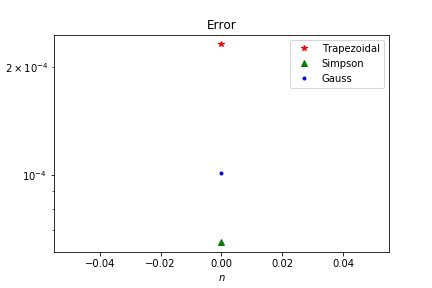
\includegraphics[scale=.7]{7err.png}
\end{center}
If we consider the effects of $n$ on the accuracy, we see that Simpson's method remains the most accurate after the initial few values of $n$.  
\begin{center}
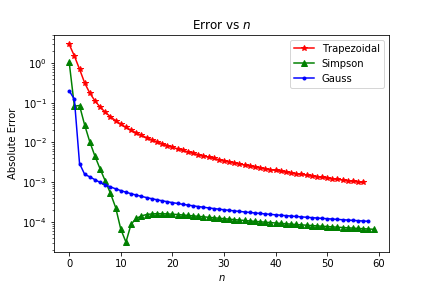
\includegraphics[scale=.7]{7allerr.png}
\end{center}
\end{enumerate}
\item We consider the Legendre polynomial $P_2(x)=3x^2-1$, as well as $p(x)=6x^3+5x^2+x$.
\begin{enumerate}
\item Let $Q(x)=ax+b$, and consider,
\begin{align*}
\int_{-1}^{1}P_2(x)Q(x)dx &= \int_{-1}^1(3x^2-1)(ax+b) dx\\
&=\int_{-1}^13ax^3+3bx^2-ax-b dx\\
&=\left[\frac{3ax^4}{4}+bx^3-\frac{ax^2}{2}-bx\right]\bigg|_{-1}^1\\
&=\left(\frac{3a}{4}+b-\frac{a}{2}-b\right)-\left(\frac{3a}{4}-b-\frac{a}{2}+b\right)\\
&=0
\end{align*}
So, we see that for all linear polynomials, $\int_{-1}^{1}P_2(x)Q(x)dx=0$, as desired.
\item Consider now, $Q(x)=ax+b$ and $R(x)=cx+d$. We then consider,
\begin{align*}
6x^3+5x^2+x &= (3x^2-1)(ax+b)+(cx+d)\\
&=3ax^3+3bx^2-ax-b+cx+d\\
&=3ax^3+3bx^2+(-a+c)x+(-b+d)
\end{align*}
So, we arrive at the following system,
\begin{align*}
6 &= 3a \Rightarrow a=2\\
5 &= 3b \Rightarrow b=\frac{5}{3}\\
1 &= -2+c \Rightarrow c=3\\
0 &= -\frac{5}{3}+d \Rightarrow d=\frac{5}{3}
\end{align*}
So, we have the polynomials,
\begin{align*}
Q(x) &= 2x+\frac{5}{3} \\
R(x) &= 3x+\frac{5}{3}
\end{align*}
\item Consider now,
\begin{align*}
\int_{-1}^1p(x)dx &= \int_{-1}^1P_2(x)Q(x)+R(x)dx && \text{Noting that the first term is zero from part a}\\
&=0+\int_{-1}^1R(x)dx
\end{align*}
\item Finally, we consider the weights and nodes of the Gaussian Quadrature. For polynomials, we know that the quadrature results are exact to order $2n-1$ where $n$ is the number of nodes. Given that $p(x)$ is of order $3$, $n=2$ will be exact. So,
we find the nodes and weights to be,
\[x_i=\pm \frac{1}{\sqrt{3}},\ \ \ w_i=1\]
Our integral is then,
\[\int_{-1}^1p(x)=w_1R(x_1)+w_2R(w_2)=R\left(\frac{-1}{\sqrt{3}}\right)+R\left(\frac{1}{\sqrt{3}}\right)=\frac{10}{3}\]
Which is the exact solution.
\end{enumerate}
\item We consider the transformation from $[a,b]$ to $[-1,1]$.
\begin{align*}
x &\to x-a && \text{Map a to zero}\\
x-a &\to \frac{x-a}{b-a} && \text{Scale by width of original interval}\\
\frac{x-a}{b-a} &\to \frac{x-a}{b-a}(1-(-1)) && \text{Scale by width of new interval}\\
\frac{x-a}{b-a}(2) &\to 2\frac{x-a}{b-a} -1 && \text{Shift to lower end point}
\end{align*}
So our transformation is,
\[t(x)=2\frac{x-a}{b-a}-1\]
Deriving,
\[\frac{dt}{dx}=\frac{2}{b-a}\Rightarrow \frac{b-a}{2}dt=dx\]
So, our constant is $T=\frac{b-a}{2}$.
\item We now consider the $erf$ function. Using the trapezoidal rule on node counts varying from $2$ to $1024$, we compute the absolute error. The results on a semilog plot follow,
\begin{center}
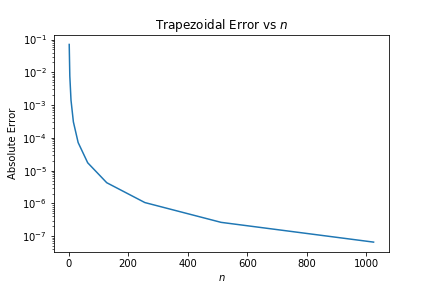
\includegraphics[scale=.7]{10trap.png}
\end{center}
We also consider using Simpson's rule to compute the error, the error plot follows.
\begin{center}
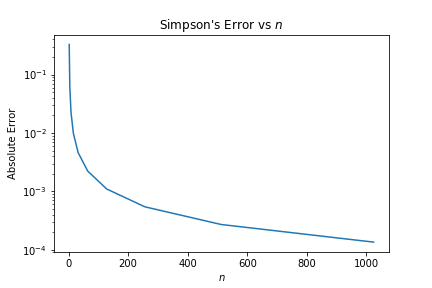
\includegraphics[scale=.7]{10simp.png}
\end{center}
Finally, we consider the following,
\[\frac{2}{\sqrt{\pi}}\int_0^1e^{-t^2}dt=\frac{2}{\sqrt{\pi}}\int_{-1}^1\frac{1}{2} e^{-((x+1)/2)^2}dx\]
Here, our scaling factor is $T=\frac{1}{2}$. We then compute the corresponding nodes and scale the weights by $T$ to compute the integral approximation. The plot of the error follows,
\begin{center}
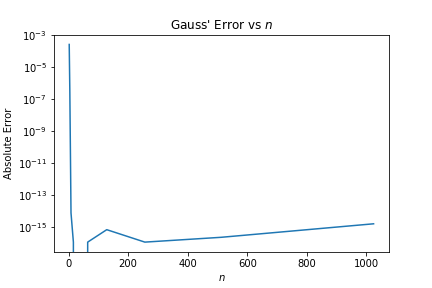
\includegraphics[scale=.7]{10gauss.png}
\end{center}
Finally, we look at the overlay of the three errors,
\begin{center}
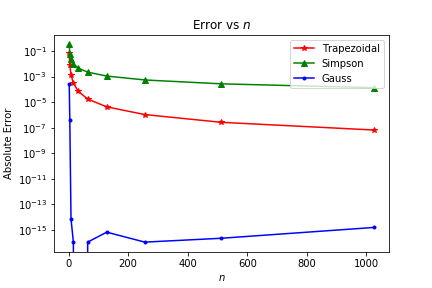
\includegraphics[scale=.7]{10allerr.png}
\end{center}
We see a very interesting behavior in the Gaussian quadrature method. It very quickly reaches an optimal value, and then starts to increase. It is possible that this is due to the error approaching machine epsilon almost immediately, and then further computations having an erroneous component. Aside from this, we notice that the trapezoidal rule performs better than Simpson's rule. This makes sense, as the $erf$ function is closely related to our standard trigonometric functions. Because the trapezoidal rule has spectral accuracy for periodic functions, we would expect it to work well for the $erf$ function as well.
\end{enumerate}
\end{document}
